\begin{figure*}[!hbt]
  \centering
  \subfigure[Speedup with varying Frontier tolerance $\tau_f$]{
    \label{fig:adjust-frontier--speedup}
    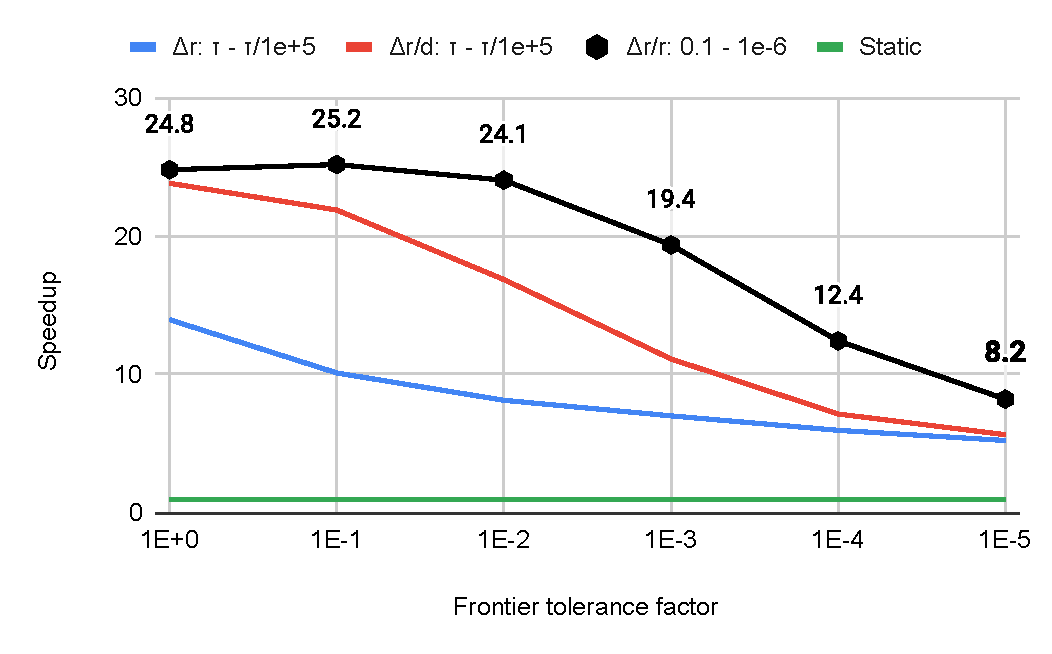
\includegraphics[width=0.48\linewidth]{out/adjust-frontier-speedup.pdf}
  }
  \subfigure[Error in ranks obtained with varying Frontier tolerance $\tau_f$]{
    \label{fig:adjust-frontier--error}
    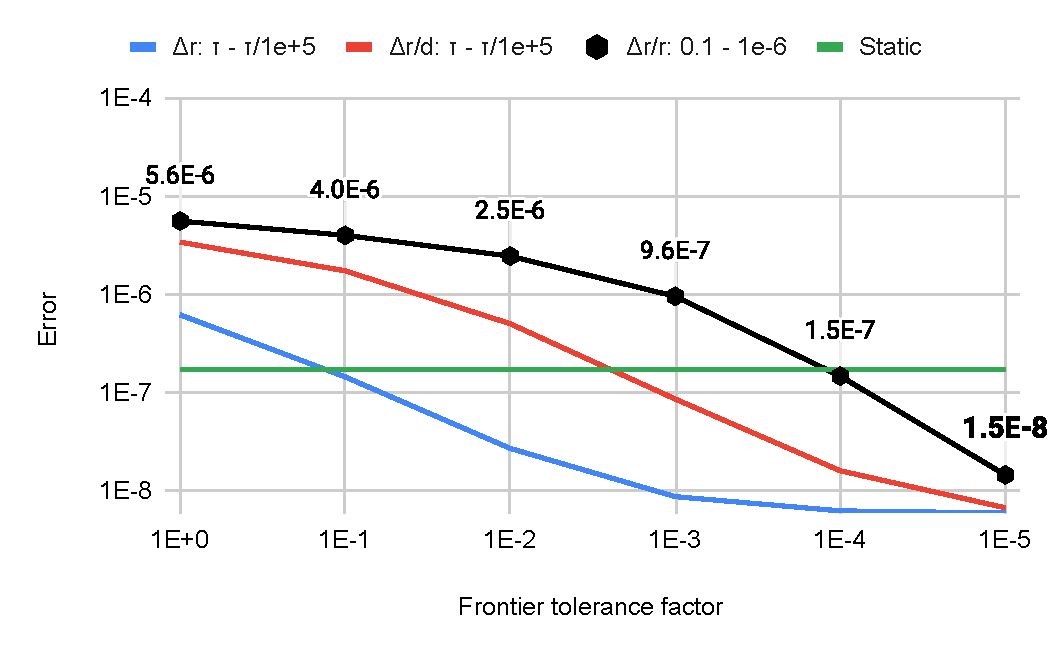
\includegraphics[width=0.48\linewidth]{out/adjust-frontier-error.pdf}
  } \\[-2ex]
  \caption{Mean Speedup and Error in ranks obtained with three different frontier expansion approaches: Change in rank ($\Delta r$), Change in contribution factor ($\Delta r/d$), and Relative change in rank ($\Delta r/r$). Here, $\Delta r$ represents the change in rank of a vertex, $d$ is its out-degree, and $r$ is the maximum of the previous and current rank value of the vertex. For the first two approaches, we adjust the frontier tolerance $\tau_f$ from $\tau$ to $\tau/10^5$ ($\tau$ is iteration tolerance), and for the last approach, we adjust it from $0.1$ to $10^{-6}$. With each approach, we mark outgoing neighbors as affected if the defined metric exceeds $\tau_f$. We also include the mean speedup and error in ranks obtained with Static PageRank as a reference. This figure demonstrates that the $\Delta r/r$ approach with a $\tau_f$ of $10^{-6}$ performs the best, while achieving ranks with lower error than Static PageRank.}
  \label{fig:adjust-frontier}
\end{figure*}

\ignore{Mean Speedup and Error in ranks obtained (with respect to ranks obtained with Reference Static PageRank) with three different approaches of expanding frontier, i.e., marking outgoing neighbors as affected, based on: Change in rank $\Delta r$, Change in contribution factor $\Delta r/d$, and Relative change in rank $\Delta r/r$ of a vertex. Here, $\Delta r$ is the change in rank of a vertex, $d$ is its out-degree, and $r$ represents the rank of the vertex (it is actually the \texttt{max} of the previous and the current rank value of the vertex). For the first two approaches for expanding frontier, i.e., $\Delta r$ and $\Delta r/d$, we adjust the frontier tolerance $\tau_f$ from $\tau$ to $\tau/10^5$ (where $\tau$ is the iteration tolerance), and for the last approach, i.e., $\Delta r/r$, we adjust the frontier tolerance from $0.1$ to $10^-6$ (note that the $0.1$ beside $\Delta r/r$ indicates that the frontier tolerance $\tau_f$ starts from $0.1$). With each approach, we mark the outgoing neighbors of a vertex as affected, only if the metric/measure defined by the approach exceeds the frontier tolerance $\tau_f$. We also include the mean speedup ($1$) and error in ranks obtained ($1.7\times10^{-7}$) with Static PageRank as a reference. This figure indicates that the $\Delta r/r$ approach with a frontier tolerance $\tau_f$ of $10^{-6}$ (i.e., frontier tolerance factor of $10^{-5}$) performs the best, while obtaining ranks with lower error than Static PageRank.}
